\chapter{Choix du type d'algorithme}
Ce dataset contient des informations sur l'ensemble des courses de Formule 1 depuis l'année 1950. Il y a plusieurs fichiers des datas sur les pilotes, les tracées des courses, sur les écuries, et l'emble des résultats pour les qualifications, course sprint et (vrai) course. Le fichier le plus important est result.csv car il contient les résultats de chaque course avec le score de chaque pilote et le lieux. L'objectif est de trouvé un modèle qui permet de prédire le nombre de point d´un pilote à la fin d'une saison. Pour cela, nous devons trouver les variables qui ont le plus d'impact sur le nombre de point d´un pilote. Il s'agit d'un apprentissage supervisé car nous avons un jeu de données d'entraînement et un jeu de données à tester. Nous devons prédire un nombre de point d'un pilote à la fin d´une saison. Je pense qu'il faut utiliser une régression parce que nous devons déterminer une valeur numérique.

\section{Algorithme 1 : Algorithme de régression linéaire simple}
J'ai commencé par analyser mes données et sélectionner celle qui me semble importante pour commencer. En premier lieux j'ai commencé par une régression linéaire simple pour prendre en main les différentes bibliothèques. J'ai pris comme paramètre le nombre de points d'un pilote par rapport à ses différentes courses. Les résultats ne sont pas très concluant car le modèle n'est pas très précis. Le nombre de points gagné par un pilote sur une course ne dépend pas uniquement du tracé d'un circuit.

\section{Algorithme 2 : Algorithmes de régression linéaire logistique}
J'avais entendu parler de la régression linéaire logistique, cependant, après des premières recherches, elle ne semble pas correspondre à mon problème. En effet, celle ci est principalement utilisé pour une classification binaire. Notre problème est de déterminer le nombre de points gagner et cela n'est pas un choix entre deux solutions prédéfinis.

\newpage
\section{Choix d'un meilleur algorithme}

\href{https://scikit-learn.org/stable/tutorial/machine_learning_map/index.html}{Cheat-Sheet de Sckit-Learn}\\

\begin{figure}[H]
    \centering
    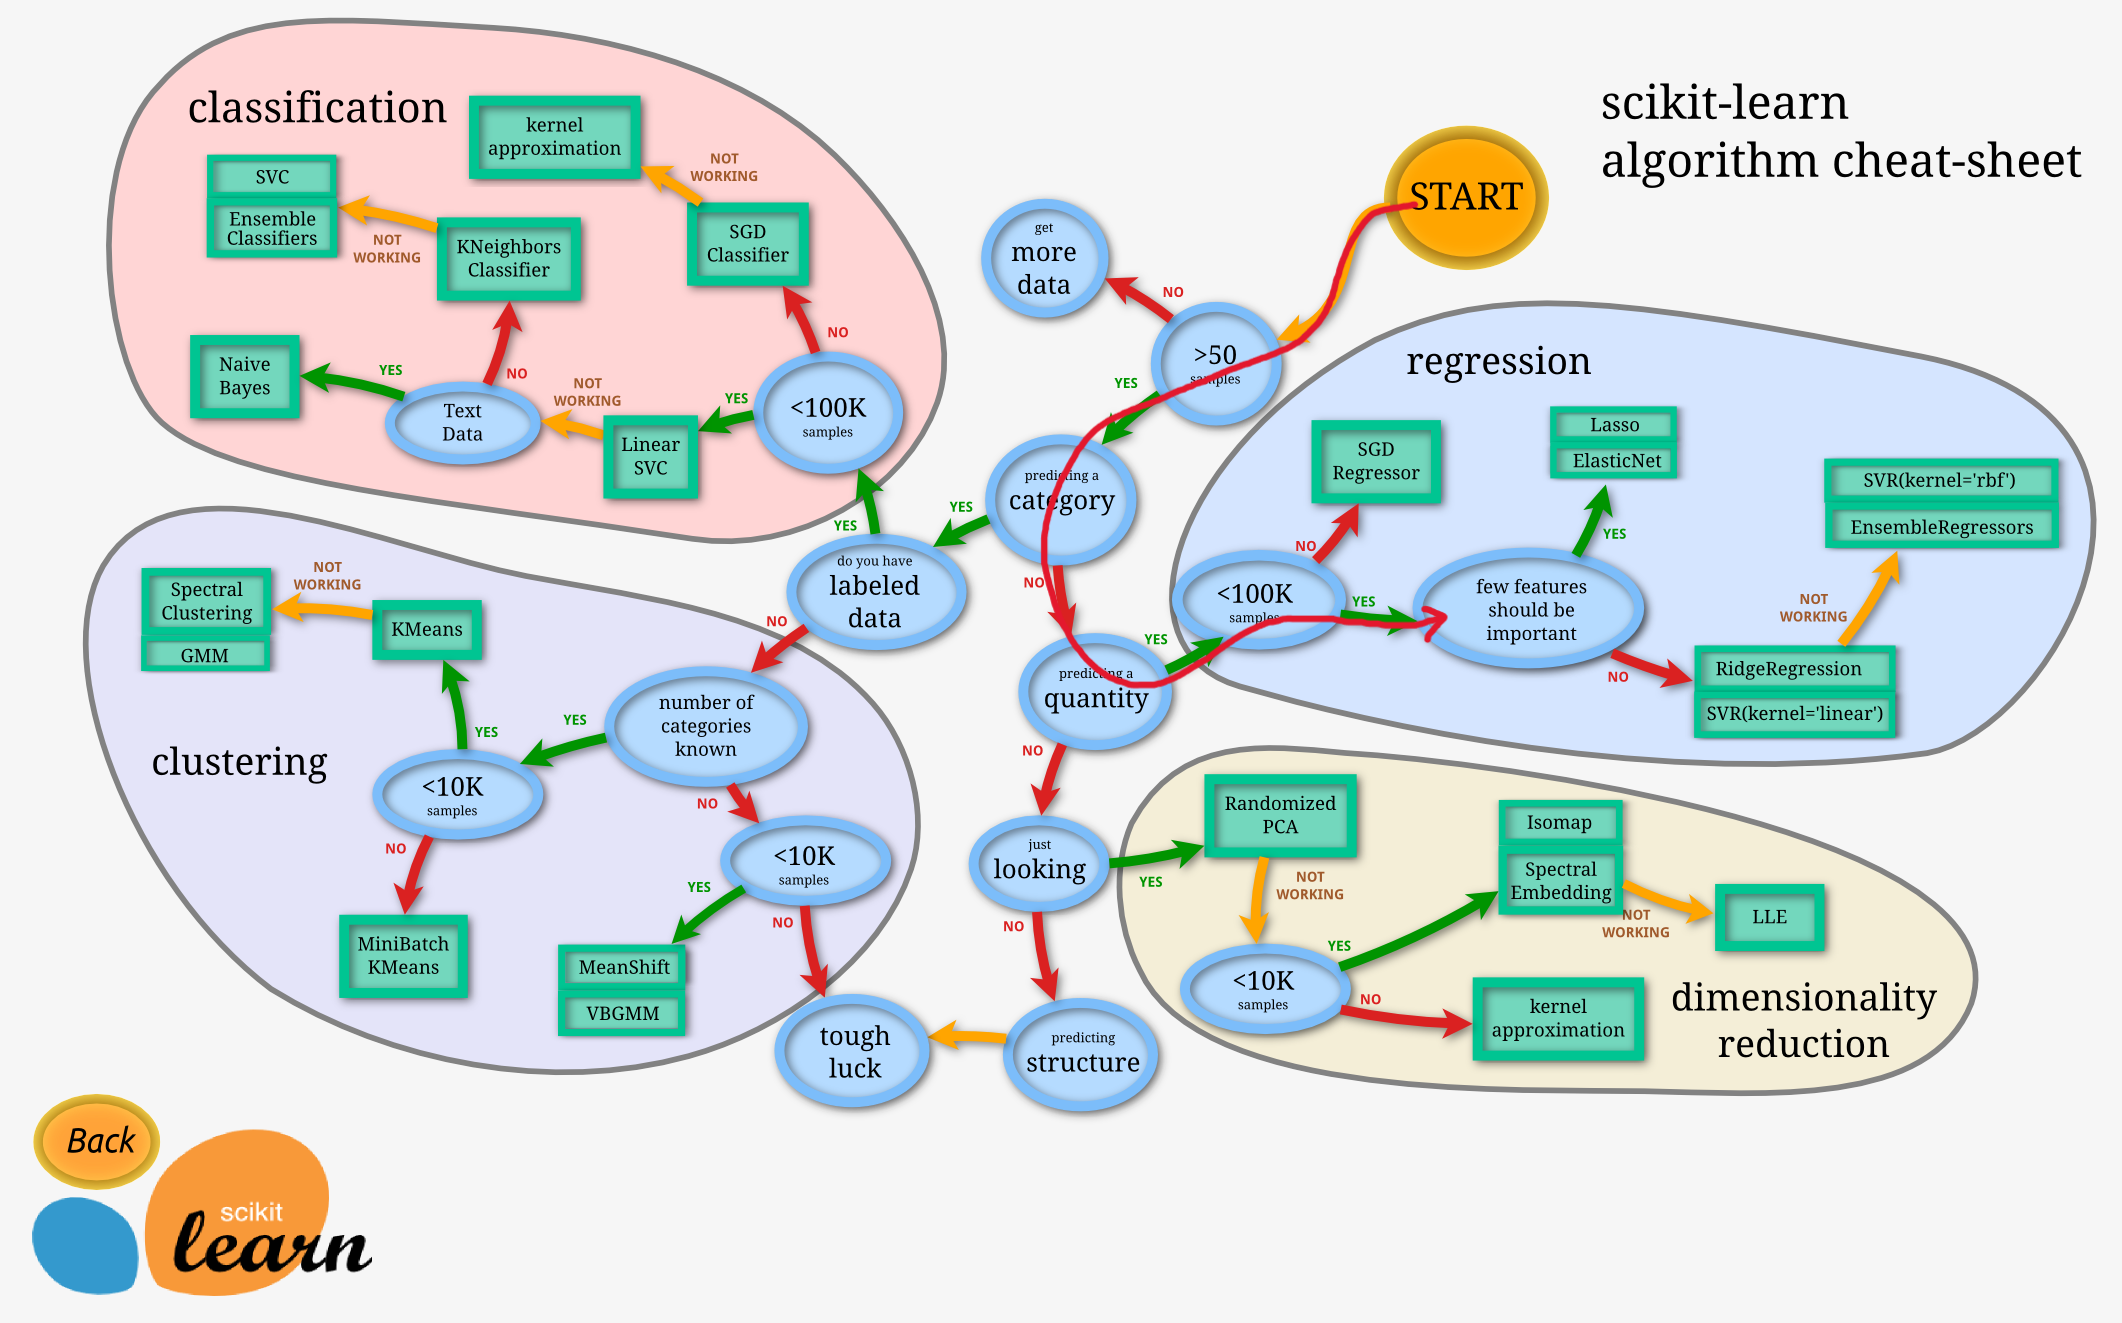
\includegraphics[width=1\textwidth]{images/cheat-sheet.png} 
    \caption{Chemin choisit pour mon projet sur la Cheat-Sheet}
\end{figure}
Étant données qu'aucun des premiers algorithmes étaient intéressant au vu des résultats à cause principalement du fait qu'il ne prend qu'un seul paramètre en entrée. Je me suis donc dirigée vers la cheat-sheet de scikit-learn qui nous permet de déterminer quelle algorithme utiliser pour tenter d'atteindre notre objectif de prédiction. Nous avons déjà plus de 50 exemples et ne nous cherchons pas à prédire une catégorie. Ensuite nous voulons prédire une quantité et nous avons moins de 100 000 exemples, ce qui mène au dernier choix qui nous demande si peu de caractéristiques devraient être importante ou non. Nous cherchons donc a réaliser une régression et pour ce dernier choix, je vais faire des tests avec les différents algorithmes proposé pour chacun d'eux avec l'algorithme Lasso et la RidgeRegression. En effet ces deux algorithmes permettent de prendre plusieurs paramètre en entier afin que le résultat en sortit soit plus réaliste. Dans un Grand-prix de F1, ce n'est pas seulement sa position de dé part ou juste l'équipe à laquelle appartient un pilote, qui permet de savoir le nombre de points que va obtenir un pilote à a fin de la course, mais plutôt un ensemble de facteurs combinés. 

\section{Algorithme de régression LASSO}

Le premier algorithme de régression prenant plusieurs paramètre en entrée que je vais étudier est un algorithme de regression LASSO pour Least Absolute Shrinkage and Selection Operator et qui me permet de choisir les paramètres les plus importants dans l'ensemble de mes fichiers. En effet, pour prédire le nombre de points qu'un pilote de Formule 1 peut gagner, cet algorithme permet de sélectionner automatiquement les variables les plus importantes pour la prédiction. Dans le cas de la Formule 1, il y a souvent beaucoup de variables qui peuvent influencer les performances d'un pilote, telles que l'âge, l'expérience, la vitesse moyenne, les positions de départ en pôle position, et l'ensemble des points déjà gagner par grand-prix. Le fait d'utiliser une régression Lasso pour sélectionner les paramètres les plus intéressants pourrais améliorer la précision des prédictions et éviter le sur-apprentissage.

